\documentclass{swp1}
\usepackage[utf8]{inputenc}
\usepackage{amssymb}
\usepackage{url}


% Tabellen
\usepackage{tabularx}
\usepackage{supertabular}
\usepackage{booktabs}







\begin{document}

% \maketitle{Nummer}{Abgabedatum}{Tutor-Name}{Gruppennummer}
%           {Teilnehmer 1}{Teilnehmer 2}{Teilnehmer 3}
\maketitle{4}{13.07.2014}{Michaela Bunke}{ChronoX}
          {Tim Ellhoff}{Karsten Betjemann}{}
          
\section*{Aufgabe 1)}

\begin{figure}[h]
\centering{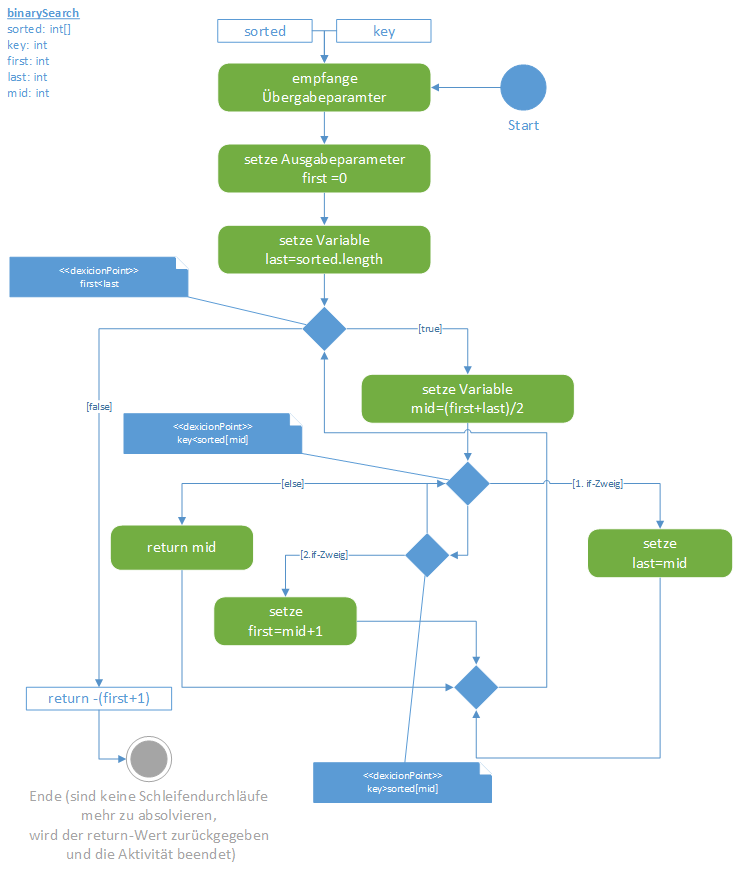
\includegraphics[width=13cm]{aufg1.png}}
\caption{Kontrollfluss der Java-Methode \texttt{binarySearch} in einem Aktivitätsdiagramm dargestellt}
\label{ab1}
\end{figure}


\section*{Aufgabe 2)}
\section*{Aufgabe 3)}
\section*{Aufgabe 4)}

********ALLES NOCH IN BEARBEITUNG...........\\

Dargestellt ist der Ablauf in einem Online-Shop, visualisiert in einem Sequenzdiagramm. Dabei regelt die Klasse \texttt{ShoppingSession} die Shop-Sitzung und ist ebenso für die Darstellung des Shops zuständig. Die Klasse \texttt{Cart} stellt einen Einkaufswagen dar und die Klasse \texttt{ProductDB} repräsentiert den Zugriff auf die Produktdatenbank.

\textbf{Beschreibung des abgebildeten Vorgangs:}\\
Der Kunde ruft zunächst den Online-Shop auf. Es wird dabei eine Shop-Sitzung erstellt. Er sucht ein Notebook. Dazu gibt er in einem Suchfeld das Stichwort \glqq Notebook\grqq ein. 

\textbf{Äquivalentes Kommunikationsdiagramm:}\\


\end{document}

